\section[Měření kinetických parametrů]{Kinetické parametry reaktoru, zpožděné neutrony, jejich vlastnosti, vliv na provoz reaktoru a určování jejich parametrů}

\subsection{Kinetické parametry reaktoru}
Kinetika rektoru zkoumá časové chování reaktoru se změnou vstupních parametrů, přičemž vstupními parametry primárně chápeme $k_\text{ef}$, který lze ovlivnit změnou geometrie, či materiálového složení. 

K popisu kinetiky reaktoru lze využít transportní rovnici, resp. zjednodušenou difúzní rovnici $\rightarrow$ vede na komplikované soustavy, které nelze v obecném případě řešit analyticky (s projevem heterogenity systému).

V praxi se využívají zjednodušené rovnice kinetiky, tzv. \textbf{Rovnice bodové kinetiky}, které zanedbávají změnu prostorového rozložení $\rightarrow$ nastane-li změna na vstupních parametrech (zvětší-li se reaktivita), tak změna výstupních parametrů (např. $\phi$) se ve všech místech změní stejnou měrou $\rightarrow$ výstupní parametry se tedy pouze škálují a průběh zůstává zachován. Kromě prostorové závislosti se zanedbává i energetické rozdělení $\rightarrow$ vede na 1G rovnice.

V reálu to tak není, ale kupodivu dávají rovnice přijatelné výsledky.

\subsection{Rovnice jednobodové kinetiky}
Pro odvození se vychází z 1G difúzní rovnice (s konstantním $D$ a $\Sigma_a$). Po sérii úprav a zanedbání se dostáváme na tvar: (Odvození je popsáno jinde :D).

Destrukční tvar rovnic:
\begin{equation}
  \boxed{
  \dfrac{dN}{dt} = \dfrac{k_{\text{ef}}(1-\beta_{\text{ef}})-1}{\ell} N(t) + \sum_{i=1}^m \lambda_i C_i(t),
  \label{rovnice_kinetiky_zpozdenky_1}}
\end{equation}

\begin{equation}
  \boxed{
  \dfrac{dC_i}{dt} = -\lambda_i C_i(t) + \dfrac{\beta_{\text{ef},i} k_{\text{ef}} N(t)}{\ell},
  \label{rovnice_kinetiky_zpozdenky_2}}
\end{equation}

Produkční tvar rovnic:
\begin{equation}
  \boxed{
  \dfrac{dN}{dt} = \dfrac{\rho - \beta_{\text{ef}}}{\Lambda} N(t) + \sum_{i=1}^m \lambda_i C_i(t),
  \label{rovnice_kinetiky_zpozdenky_3}}
\end{equation}

\begin{equation}
  \boxed{
  \dfrac{dC_i}{dt} = -\lambda_i C_i(t) + \dfrac{\beta_{\text{ef},i}  N(t)}{\Lambda}.
  \label{rovnice_kinetiky_zpozdenky_4}}
\end{equation}

\subsection{Kinetické parametry}
K popisu rovnic jednobodové kinetiky bylo využito parametrů, které budou popsány níže.

\textbf{Střední doba života neutronů} -  $\ell$ (s)

\begin{equation}
  \boxed{
  \ell \equiv \dfrac{1}{v \Sigma_a} \dfrac{1}{1+L^2B_g^2}
  \label{stredni_doba_zivota}}
\end{equation}

\begin{table}[H]
\small
\centering
\caption{\small Střední doby života pro různé typy reaktorů.}
\label{table_stredni_doby_zivota}
\begin{tabular}{@{}rc@{}}
\toprule
\textbf{Typ systému} & $\ell$ (s)           \\ \midrule
\textbf{FR}          & $10^{-7}$            \\
\textbf{LWR}         & $10^{-5} - 10^{-4}$  \\
\textbf{Grafit}      & $10^{-3}$            \\ \bottomrule
\end{tabular}
\end{table}

\textbf{Efektivní střední doba života neutronů} -  $\ell^*$ (s) \\
Tohle už bere do úvahy i zpožděnky a lze podle toho definovat další "efektivní" kinetické parametry
\begin{equation}
  \boxed{
  \ell^* \equiv \ell(1-\beta) + \sum_i \beta_i \tau_i,
  \label{efektivni_stredni_doba_zivota}}
\end{equation}

\textbf{Perioda reaktoru} - $T_e$ (s) \\
Zadefinujeme si \textbf{periodu reaktoru} $T_e$ (s) jako dobu, za kterou se výkon v systému změní e-krát, pomocí vztahu:

\begin{equation}
  \boxed{
  T_e \equiv \dfrac{\ell}{k_{\text{ef}} - 1}.
  \label{perioda}}
\end{equation}

\textbf{Střední doba vzniku neutronů} - $\Lambda$ (s) \\
Je definována jako průměrná doba mezi emisí neutronu v jednom štěpení a jeho absorbováním nebo způsobením dalšího štěpení. Nižší hodnota $\Lambda$ znamená rychlejší dynamickou odezvu reaktoru.
\begin{equation}
  \boxed{
  \Lambda \equiv \dfrac{\ell}{k_{\text{ef}}}.
  \label{stredni_doba_vzniku}}
\end{equation}

\textbf{Podíl zpožděných neutronů} - $\beta$ (-)

\begin{equation}
  \boxed{
  \beta \equiv \dfrac{\nu_D}{\nu_T},
  \label{zpozdenky}}
\end{equation}

kde:

\begin{itemize}
  \item $\nu_D$ (-) značí střední počet zpožděných neutronů vzniklých při jednom štěpení,
  \item $\nu_T$ (-) značí střední počet všech vzniklých neutronů.
\end{itemize}

\begin{table}[h!]
\centering
\caption{Kinetické parametry různých izotopů.}
\label{tab:kinetic_parameters}
\begin{tabular}{ccccccc}
\toprule
\textbf{Izotop} & $\nu_p$ (n/štěpení) & $\nu_d$ (n/štěpení) & $\nu_\text{tot}$ (n/štěpení) & $\beta$ (-) & $\overline{T}_{1/2}$ (s) & $\overline{\lambda}$ (s$^{-1}$) \\ \midrule
\textsuperscript{235}U & 2,416 & 0,0158 & 2,432 & 0,0065 & 9,022 & 0,077 \\ 
\textsuperscript{233}U & 2,475 & 0,0066 & 2,482 & 0,0027 & 12,796 & 0,054 \\ 
\textsuperscript{239}Pu & 2,868 & 0,0061 & 2,874 & 0,0021 & 10,672 & 0,065 \\ \bottomrule
\end{tabular}
\end{table}

\textbf{Efektivní podíl zpožděných neutronů} - $\beta_\text{ef}$ (-)\\
Umělá hodnota, která koriguje energetický rozdíl ve skupinách, jelikož každá ze skupin má jiný vliv na štěpeni. Lze ji zavést pomocí vztahu:

\begin{equation}
  \beta_{\text{ef}} = \beta \cdot I,
\end{equation}

kde $I$ (-) značí tzv. \textbf{funkci vlivu} a závisí na konkrétním reaktoru. Říká, jak je snadné pro zpožděné neutrony štěpit, oproti okamžitým neutronům. Obecně se pohybuje okolo $\approx 1$, při bližším studiu lze napsat: FR $<1$ a LWR $>1$.\\


\subsection{Zpožděné neutrony}

Kinetika a dynamika jaderného reaktoru v průběhu jeho provozu (především při přechodových procesech) je do značné míry udávána zpožděnými neutrony. Znalost parametrů zpožděných neutronů je velmi významná nejen při návrhu, ale i vlastním provozu jaderných reaktorů. Zpožděné neutrony lze využít také jako analytický nástroj, pomocí něhož lze přesněji určit obohacení, respektive hmotnost štěpného materiálu.

Z hlediska řízení reaktivity platí, že nikdy nesmí dojít ke kritičnosti na okamžitých neutronech, jelikož se tím drasticky (až o několik řádů) sníží perioda reaktoru, viz otázky FJR. Rovněž více o kinetických parametrech reaktoru je k dohledání v otázkách FJR, případně ve wikiSkriptech z KIDu

\subsubsection{Vznik a vlastnosti zpožděných neutronů}

Štěpení spočívá v rozdělení jádra (např. $^{235}\text{U}$) na dva nebo více úštěpků s hmotnostmi a atomovými čísly podstatně menšími než u výchozího jádra. V prvním stádiu štěpné reakce dochází k pohlcení neutronu, přičemž vznikne jádro $^{236}\text{U}$ ve vzbuzeném stavu:

\[
^{235}_{92}\text{U} + \text{n} \rightarrow ^{236}_{92}\text{U}^*
\]

Takto vzniklé jádro může emitovat gama záření a přejít tak do základního stavu nebo může dojít k jeho rozštěpení. 

Produkty štěpení mají příliš vysoký poměr počtu neutronů k počtu protonů a jsou tedy nestabilní. Proto téměř všechny produkty štěpení jsou radioaktivní a dochází u nich nejčastěji k rozpadu $\beta^-$ se spojeným zářením gama. Radioaktivní bývají i přímé produkty rozpadu, u nichž může opět docházet k rozpadu $\beta^-$, než vznikne stabilní jádro. Délka rozpadových řad bývá různá, v průměru procházejí produkty štěpení třemi rozpadovými stádii, než se utvoří stabilní jádro. V některých případech vede rozpad $\beta^-$ jádra, které se nachází ve vzbuzeném stavu, k uvolnění neutronu. Jelikož energie vázaného neutronu je nižší než vazbová energie neutronu v jádře, pak je určitá pravděpodobnost, že dojde k emisí neutronu a vzniku stabilního jádra. Uvolněný neutron se nazývá zpožděným neutronem. Zpoždění je dáno pouze poločasem rozpadu produktu štěpení, který je nazýván prekurzorem, jelikož k uvolnění neutronu dochází až po předchozím rozpadu jeho jádra.

Obecně lze zapsat vznik zpožděného neutronu následujícím předpisem:

\[
^A_Z\text{X} \xrightarrow{\beta^-} {}^{A}_{Z+1}\text{Y} \rightarrow ^{A-1}_{Z+1}\text{Y} + \text{n}
\]

kde:

\begin{itemize}%[noitemsep]
    \item $^A_Z\text{X}$ je produkt štěpení, jádro nazývané prekurzor neboli předchůdce mateřského jádra,
    \item $^{A}_{Z+1}\text{Y}$ je jádro nazývané emitor neboli mateřské jádro,
    \item $^{A-1}_{Z+1}\text{Y}$ je výsledné jádro.
\end{itemize}

Na Obrázku \ref{SNM} je znázorněno rozpadové schéma typického prekurzoru $^{87}\text{Br}$. Izotop $^{87}\text{Br}$ hraje významnou roli v případě odstavení jaderného reaktoru, kdy odezní vliv okamžitých a krátkodobě žijících zpožděných neutronů. V tomto případě je populace neutronů v AZ určována především rozpadem $^{87}\text{Br}$. Jak vyplývá z obrázku, přibližně 30~\% jader $^{87}\text{Br}$ přechází rozpadem $\beta^-$ na $^{87}\text{Kr}$, který se nachází v základním stavu, zatímco 70~\% jader přechází rozpadem $\beta^-$ na $^{87}\text{Kr}$ ve vzbuzeném stavu ($^{87}\text{Kr}^*$). Z těchto 70~\% přechází přibližně 20~\% jader $^{87}\text{Kr}^*$ izomerickým přechodem do základního stavu. Zbýlá jádra ($^{87}\text{Kr}^*$) se dostávají do základního stavu přímou emisí neutronu. Tím vzniká zpožděný neutron. Prekurzorem je tedy $^{87}\text{Br}$, který opět rozpadem $\beta^-$ přechází na již stabilní $^{87}\text{Sr}$. Zpožděný neutron není emitován přímo jádrem $^{87}\text{Br}$, ale dceřiným produktem ve vzbuzeném stavu ($^{87}\text{Kr}^*$).

\begin{figure}[H] 
    \centering
    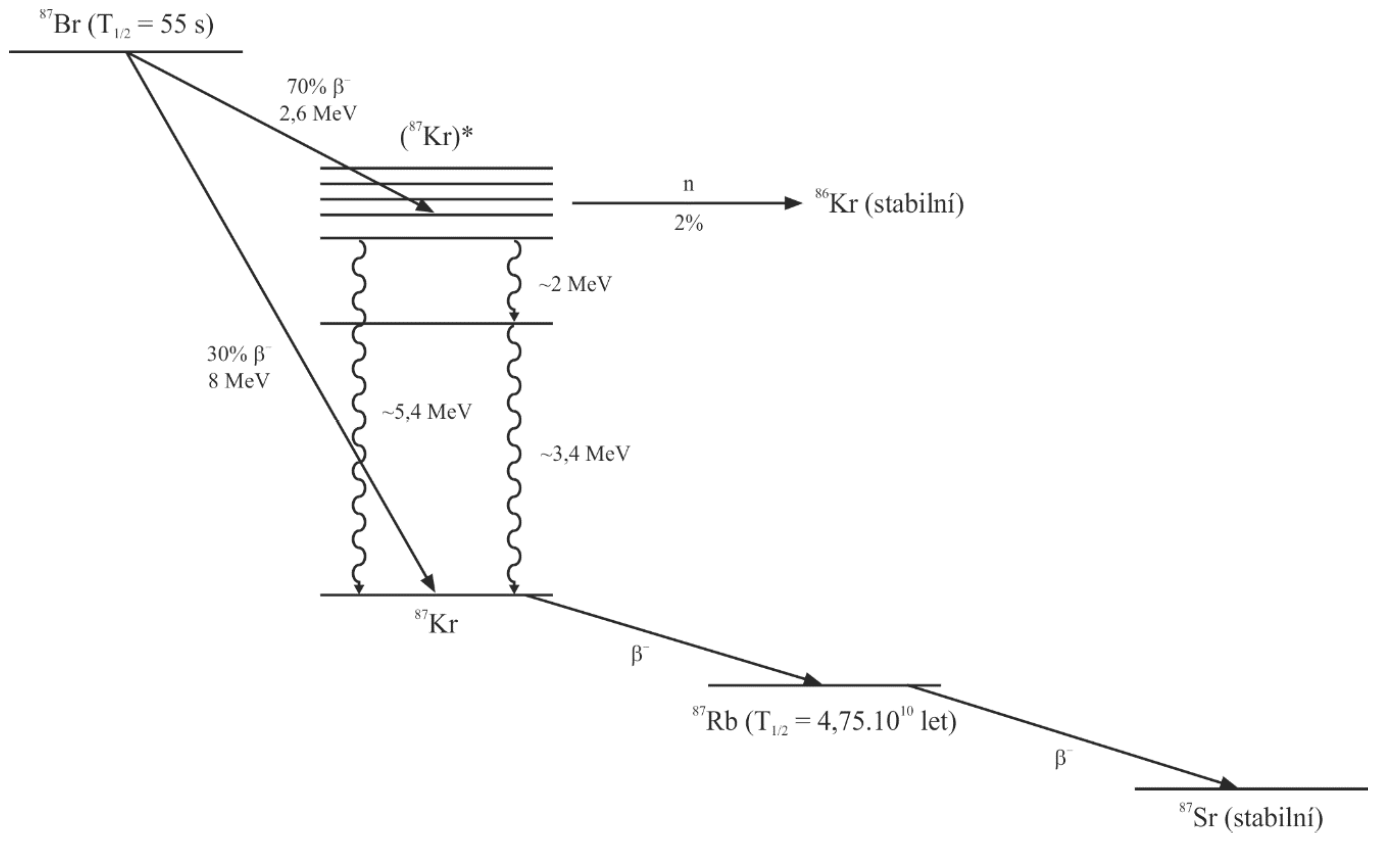
\includegraphics[width=0.8\textwidth]{img/ZpožděnéNeutrony.png}
    \caption{Rozpadové schéma $^{87}$Br.}
    \label{SNM}
\end{figure}

V současnosti bylo identifikováno téměř 400 prekurzorů zpožděných neutronů. Nejdéle žijícími jsou $^{91}\text{Rb}$ a $^{87}\text{Br}$ s poločasem rozpadu 58,4~s, respektive 55,6~s, zatímco $^{102}\text{Rb}$ a $^{101}\text{Rb}$ jsou krátkodobě žijící prekurzory s poločasem rozpadu 37~ms, respektive 32~ms. Jelikož k emisi neutronu dochází bezprostředně po rozpadu prekurzoru, řídí se časové zpoždění, s nímž se emitované neutrony objevují, zákony radioaktivního rozpadu těchto jader.

Jelikož prekurzorů je moc, tak se pro optimalizaci výpočtů prekurzory slučují do několika skupin, přičemž každá skupina je charakteristická jedním středním poločasem rozpadu a jedním společným kumulativním výtěžkem. Čím více skupin, tím přesnější výpočet, ale tím složitější a zdlouhavější výpočet. Pro první přiblížení stačí použít 1-2 skupiny, lepší kódy aplikují 6-8 skupin (záleží na knihovně, např. ENDF/B má 6 skupin a JEFF 8 skupin).

\begin{table}[H]
    \centering
    \begin{tabular}{@{}ccc@{}}
    \toprule
    Skupina & Prekurzor                              & T$_{1/2}$ (s) \\ \midrule
    1       & $^{87}$Br, $^{142}$Cs                  & 55,72         \\
    2       & $^{137}$I, $^{88}$Br                   & 22,72         \\
    3       & $^{138}$I, $^{89}$Br                   & 6,22          \\
    4       & $^{139}$I, $^{(93, 94)}$Kr, $^{143}$Xe & 2,30          \\
    5       & $^{140}$I, $^{145}$Cs                  & 0,61          \\
    6       & Br, Rb, As…                            & 0,23          \\ \bottomrule
    \end{tabular}
\end{table}

Kumulativní výtěžek označovaný jako $\beta$ se pohybuje v desetinách procenta, záleží, který izotop se štěpí. Pro $^{235}$U je to asi 0,7 \%, pro izotopy Pu je to méně. Proto jsou MOXové vsázky citlivější na změnu výkonu.

Kromě výše uvedených parametrů je důležitou charakteristikou zpožděných neutronů i jejich energie. Ta se pohybuje pro jednotlivé skupiny zpožděných neutronů v rozmezí od 200~keV do 700~keV. Porovnáme-li tento rozsah energií se střední energií okamžitých neutronů (2,2~MeV), je zřejmé, že zpožděné neutrony musí v rámci zpomalovacího procesu projít menším rozsahem energií než neutrony okamžité. Je nižší pravděpodobnost, že dojde k jejich ztrátě v důsledku úniku nebo parazitické absorpce, než v případě okamžitých neutronů. Naopak u okamžitých neutronů je vyšší pravděpodobnost, že vyvolají štěpení ve vyšší oblasti energií (např. na $^{238}\text{U}$). Tyto dva efekty mají tendenci působit navzájem proti sobě, nicméně je obvykle mezi nimi určitý, i když mírný, rozdíl. V důsledku toho se definuje tzv. efektivní podíl zpožděných neutronů $\beta_\text{ef}$, který zohledňuje rozdílnou energii zpožděných neutronů oproti neutronům okamžitým a tím i jejich význam v procesu štěpení. Je tedy závislý na typu reaktoru, moderaci apod.

\subsubsection{Emise zpožděných neutronů}

Emise zpožděných neutronů je spojena se vznikem a aktivitou jejich jednotlivých mateřských jader. Vznik konkrétního prekurzoru zpožděných neutronů v průběhu ozařování můžeme popsat bilanční rovnicí ve tvaru:

\[
\frac{dN_i}{dt} = Y_C \cdot \Sigma_f \cdot \Phi - \lambda_i \cdot N_i
\]

kde:

\begin{itemize}%[noitemsep]
    \item $N_i$ je počet mateřských jader zpožděných neutronů $i$-tého druhu,
    \item $Y_C$ je kumulativní výtěžek mateřských jader zpožděných neutronů ze štěpení,
    \item $\Sigma_f$ je reakční rychlost pro štěpení,
    \item $\Phi$ je hustota toku neutronů,
    \item $\lambda_i$ je rozpadová konstanta mateřských jader zpožděných neutronů.
\end{itemize}

Pro jednoduchost je zanedbán záchyt neutronů mateřskými jádry zpožděných neutronů. Tuto rovnici lze jednoduše řešit pro $N_i$ jako funkci času ozařování:

\[
N_i(t) = \frac{Y_C \cdot \Sigma_f \cdot \Phi}{\lambda_i} \cdot \left(1 - e^{-\lambda_i t}\right).
\]

Abychom získali emisi zpožděných neutronů (tj. zdrojový člen), je nutné vynásobit obě strany rozpadovou konstantou $\lambda_i$. Za předpokladu, že mateřské jádro prochází rozpadem vedoucím k emisi neutronu $P_i$, předpokládáme-li, že druhů mateřských jader a ozářovacích časů je $t_\text{irr}$, pak počet zpožděných neutronů emitovaných v čase $t$ po ukončení ozařování bude:

\[
N_{DN}(t) = \sum_{i=1}^{m} P_i \cdot Y_C \cdot \Sigma_f \cdot \Phi \cdot (1 - e^{-\lambda_i t_\text{irr}}) \cdot e^{-\lambda_i t}.
\]

V souladu s teorií lze zpožděné neutrony rozdělit do šesti skupin podle typických mateřských jader a vztah přepsat na tvar:

\[
N_{DN}(t) = \sum_{i=1}^{6} a_i \cdot (1 - e^{-\lambda_i t_\text{irr}}) \cdot e^{-\lambda_i t},
\]

kde $a_i$ je zastoupení $i$-té skupiny zpožděných neutronů. Bude-li provedeno pouze krátkodobé ozařování (např. neutronovým pulzem), pak rovnice nabývá tvar:

\begin{equation}
    \boxed{N_{DN}(t) = \sum_{i=1}^{6} a_i \cdot e^{-\lambda_i t}.}
\end{equation}

Je-li doba ozařování dostatečně dlouhá ($t_\text{irr} \gg \tau_i$), přechází rovnice na tvar:

\begin{equation}
    \boxed{N_{DN}(t) = \sum_{i=1}^{6} a_i \cdot (1 - e^{-\lambda_i t}).}
\end{equation}

\subsubsection{Stanovení poločasu rozpadu prekurzorů zpožděných neutronů}

V případě, že bychom chtěli určit parametry jednotlivých skupin zpožděných neutronů a celkovou emisi rozdělit na individuální rozpadové křivky, je nutné aplikovat na analyzovaná data metody \textbf{nelineární regrese}. Takováto úloha není jednoduchá a pro její řešení jsou běžně používány sofistikované softwarové nástroje pro analýzu dat. Nicméně úloha se výrazně zjednoduší, pokud se bude jednat o hledání parametrů pouze jedné exponenciální funkce. Toho lze dosáhnout, pokud si uvědomíme, že platí $\lambda_1 \ll \lambda_2 \ll \dots \ll \lambda_6$ a $e^{-\lambda_1 t} \gg e^{-\lambda_2 t} \gg \dots \gg e^{-\lambda_6 t}$. Po dostatečně dlouhé době, která vede k rozpadu předchozích skupin zpožděných neutronů, můžeme vztah aproximovat pouze jednou exponenciální funkcí odpovídající nejdéle žijící skupině zpožděných neutronů:

\[
N_{DN}(t) = a_1 \cdot e^{-\lambda_1 t}
\]

Tuto funkci lze linearizovat použitím přirozeného logaritmu:

\[
\ln N_{DN}(t) = \ln a_1 - \lambda_1 \cdot t
\]

díky čemuž můžeme jednoduše určit parametry $a_1$ a $\lambda_1$. Takto získanou teoretickou emisi odečteme od celkové emise:

\[
N_{DN}(t) - a_1 \cdot e^{-\lambda_1 t}
\]

Tento rozdíl pak představuje četnost emise pro zbývající skupiny zpožděných neutronů (2 až 6), z něhož můžeme na základě výše popsané úvahy určit parametry zpožděných neutronů druhé skupiny ($a_2$ a $\lambda_2$). Tímto způsobem bychom pokračovali až k určení parametrů skupiny zpožděných neutronů s nejkratší dobou života ($a_6$ a $\lambda_6$).

Problém nastane u krátkodobých skupin (5 a 6), jelikož jejich poločas rozpadu je tak malý, že než dojde k měření, tak se většina prekurzorů rozpadne.

\begin{figure}[H] 
    \centering
    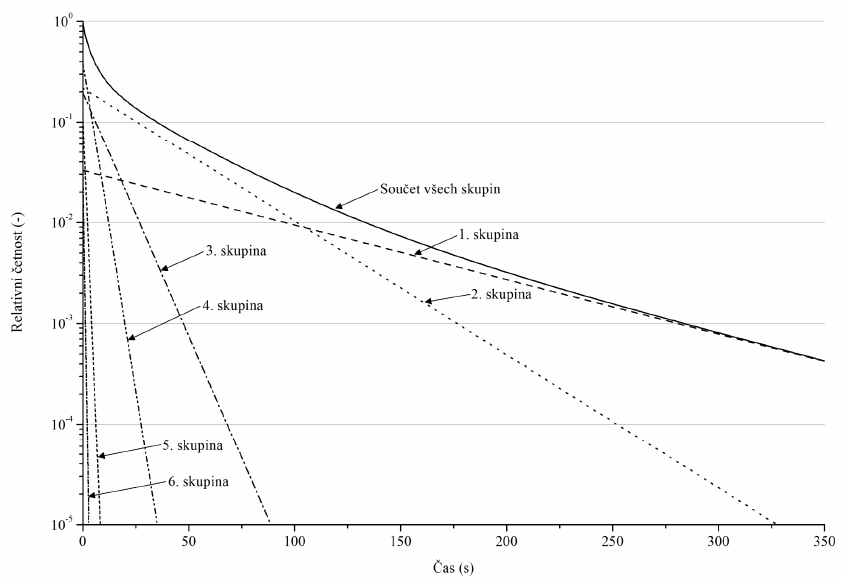
\includegraphics[width=0.8\textwidth]{img/ZpožděnéNautrony2.png}
    \caption{Měření zpožděných neutronů.}
    \label{fig:MěřeníZpožděnek}
\end{figure}

\subsubsection{Určování množství štěpného materiálu}

Z předchozí teorie je zřejmé, že celkový počet zpožděných neutronů emitovaných ozářeným štěpným materiálem závisí na počtu štěpení, což je samozřejmě spjato s množstvím jader ve štěpném materiálu. Tudíž lze využít této závislosti k určení vybraných vlastností zkoumaného vzorku, jako je množství, respektive obohacení štěpného materiálu ve vzorku.

Metoda určování množství nebo obsahu štěpného materiálu ve zkoumaném vzorku na základě detekce zpožděných neutronů je rychlá, nedestruktivní, přesná a velmi citlivá analytická metoda. Je založena na ozáření vzorku obsahujícího štěpný materiál neutrony a následné detekci zpožděných neutronů, které jsou emitovány tímto vzorkem. Množství nebo obsah štěpného materiálu ve zkoumaném vzorku je pak určená na základě porovnání intenzity zpožděných neutronů emitovaných tímto vzorkem se vzorky (standardy), u nichž je známo množství nebo obsah štěpného materiálu (za pomoci trojčlenky).

Předpokládejme zjednodušeně, že celkový počet zpožděných neutronů emitovaných ozářeným vzorkem a detekovaný detekčním systémem je roven součtu četností získaných za dobu detekce $(t_\text{end} - t_\text{start})$. Pak lze počet zpožděných neutronů $N_X$ odpovídající neznámému vzorku a počet zpožděných neutronů $N_\text{ST}$ odpovídající standardu, určit na základě následujících vztahů:

\[
N_X = \sum_{i = t_\text{start}}^{t_\text{end}} CR_{X,i}, \quad N_\text{ST} = \sum_{i = t_\text{start}}^{t_\text{end}} CR_{\text{ST},i},
\]

kde $CR_{X,i}$ a $CR_{\text{ST},i}$ jsou četnosti získané v $i$-tém časovém kroku detekčního systému pro neznámý vzorek a standard.

Je-li odezva detekčního systému na pozadí rovna:

\[
N_\text{BG} = \sum_{i = t_\text{start}}^{t_\text{end}} CR_{\text{BG},i},
\]

pak platí pro závislost počtu zpožděných neutronů produkovaných standardem na jeho hmotnosti $m_\text{ST}$ následující úměra:

\begin{equation}
m_X = m_{ST} \cdot \frac{N_X - N_\text{BG}}{N_{ST}-N_\text{BG}}.
\end{equation}

Přesnější výslednou hodnotu $m_X$ neznámého vzorku získáme, pokud použijeme více než jeden standard se štěpným materiálem. V takovém případě je vhodné vynést do grafu závislost celkového počtu zpožděných neutronů na množství štěpného materiálu, proložit data vhodnou křivkou a získat její rovnici. Z rovnice lze pak určit neznámé množství štěpného materiálu ve zkoumaném vzorku. Nicméně je důležité, aby se všemi vzorky bylo nakládáno za stejných experimentálních podmínek (hustota toku neutronů, doba ozařování, doba transportu vzorku a doba detekce) a kromě toho musí mít vzorky podobnou geometrii.

\begin{figure}[H] 
    \centering
    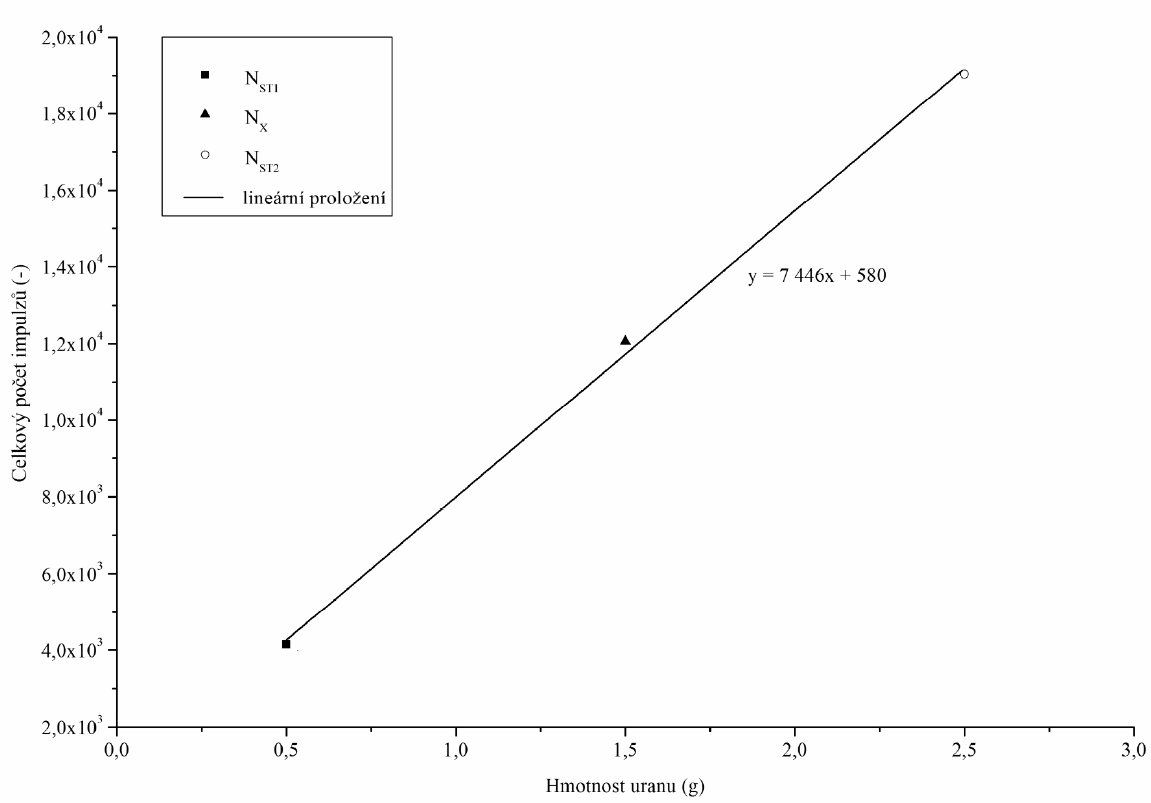
\includegraphics[width=0.8\textwidth]{img/ZpožděnéNeutrony3.png}
    \caption{Stanovení množství štěpného materiálu.}
    \label{fig:ŠtěpnýMateriál}
\end{figure}